% ============================================================
% ch03a.tex —— 第 3 章章首与 §3.1–§3.3 前半
% 原书 p.162–179（PDF p.163–180）
% 本块含 \chapter{经由伪微分算子的量子化}；§3.3 在本块末（定理 3.3.6 陈述）止，
% 其证明自原书 p.180 起，归 ch03b（tr02）
% ============================================================

% [原文 p.162]

\chapter{经由伪微分算子的量子化}

\section{傅里叶变换}

\subsection{施瓦茨函数与缓增分布}

\begin{definition}{3.1.1}
$\R^n$ 上\emph{施瓦茨函数}（Schwartz function）的空间 $S(\R^n)$，由各阶导数都速降的光滑函数组成。更确切地说，
\[
S(\R^n)=\left\{f\in C^\infty(\R^n)\ \middle|\ \|f\|_{\alpha,\beta}<\infty,\ \forall\,\alpha,\beta\right\}.
\]
这里 $\alpha=(\alpha_1,\cdots,\alpha_n)$ 与 $\beta=(\beta_1,\cdots,\beta_n)$ 是多重指标，
\[
x^\alpha:=x_1^{\alpha_1}\cdots x_n^{\alpha_n},\qquad
\partial^\beta_{x}f:=\left(\frac{\partial}{\partial x_1}\right)^{\beta_1}\cdots\left(\frac{\partial}{\partial x_n}\right)^{\beta_n}f,
\]
并且
\[
\|f\|_{\alpha,\beta}:=\sup_{x\in\R^n}\left|x^\alpha\partial^\beta_{x}f\right|.
\]
若 $\|f_k-f\|_{\alpha,\beta}\to0$ 对一切 $\alpha,\beta$ 成立，就称 $f_k\to f$ 于 $S(\R^n)$。
\end{definition}

\begin{example}{3.1.2}
设 $f$ 是 $\R^n$ 上具有紧支集的光滑函数，则 $f\in S(\R^n)$。于是
\[
C_c^\infty(\R^n)\subset S(\R^n).
\]
\end{example}

\begin{proposition}{3.1.3}
$C_c^\infty(\R^n)$ 在 $S(\R^n)$ 中稠密。
\end{proposition}

\begin{example}{3.1.4}
设 $A=(A_{ij})$ 是实对称正定的 $n\times n$ 矩阵。考虑二次多项式
\[
A(x):=\sum_{i,j=1}^n A_{ij}x^ix^j=\langle Ax,x\rangle.
\]
则对任意多项式函数 $f(x)$，
\[
f(x)e^{-A(x)}\in S(\R^n).
\]
\end{example}

% [原文 p.163]

\begin{proposition}{3.1.5}
当 $1\le p<\infty$ 时，$S(\R^n)$ 在 $L^p(\R^n)$ 中稠密。
\end{proposition}

\begin{proposition}{3.1.6}
$S(\R^n)$ 关于半范数 $\|\cdot\|_{\alpha,\beta}$ 完备。因此 $S(\R^n)$ 是\emph{弗雷歇空间}（Fréchet space）。
\end{proposition}

\begin{definition}{3.1.7}
给定 $\varphi\in S(\R^n)$，定义其\emph{傅里叶变换}（Fourier transform）
\[
\tilde\varphi(\xi)=\mathcal{F}(\varphi)(\xi):=\int_{\R^n}e^{-i\langle x,\xi\rangle}\varphi(x)\,dx.
\]
这里 $\xi=(\xi_1,\cdots,\xi_n)\in\R^n$，且 $\langle x,\xi\rangle=\sum_{i=1}^n x^i\xi_i$。
\end{definition}

\begin{theorem}{3.1.8}
傅里叶变换给出同构
\[
\mathcal{F}:S(\R^n)\longrightarrow S(\R^n),
\]
并且满足以下性质：

① \emph{傅里叶反演公式}
\[
\mathcal{F}^{-1}(\psi)(x)=\frac{1}{(2\pi)^n}\int_{\R^n}e^{i\langle x,\xi\rangle}\psi(\xi)\,d\xi.
\]
等价地，
\[
\varphi(x)=\frac{1}{(2\pi)^n}\int_{\R^n}e^{i\langle x,\xi\rangle}\tilde\varphi(\xi)\,d\xi.
\]

② \emph{微分}
\[
\mathcal{F}(D_{x}^\alpha\varphi)=\xi^\alpha\mathcal{F}(\varphi),\qquad
\mathcal{F}((-x)^\alpha\varphi)=D_{\xi}^\alpha\mathcal{F}(\varphi).
\]
这里
\[
D_{x^k}:=\frac1i\frac{\partial}{\partial x^k}=\frac{1}{\sqrt{-1}}\frac{\partial}{\partial x^k},
\qquad\text{以及}\qquad
D_{x}^\alpha:=D_{x^1}^{\alpha_1}\cdots D_{x^n}^{\alpha_n}.
\]

③ \emph{周期性}
\[
\mathcal{F}^2=(2\pi)^n\mathcal{P},\qquad\text{其中}\quad (\mathcal{P}\varphi)(x)=\varphi(-x)
\]
是\emph{宇称算子}（parity operator）。

④ \emph{共轭}
\[
\overline{\mathcal{F}(\varphi)}=\mathcal{P}\bigl(\mathcal{F}(\overline{\varphi})\bigr).
\]
\end{theorem}

\begin{example}{3.1.9}
设 $A=(A_{ij})$ 是实对称正定的 $n\times n$ 矩阵。考虑
\[
\varphi(x)=e^{-\frac12A(x)}\in S(\R^n).
\]
其傅里叶变换可按如下方式算出：
\begin{align*}
\tilde\varphi(\xi)
&=\int_{\R^n}e^{-i\langle x,\xi\rangle-\frac12A(x)}\,dx
=\int_{\R^n}e^{-\frac12\langle Ax,x\rangle-i\langle x,\xi\rangle}\,dx\\
&=e^{-\frac12\langle A^{-1}\xi,\xi\rangle}\int_{\R^n}e^{-\frac12A(x+iA^{-1}\xi)}\,dx\\
&=\frac{(2\pi)^{n/2}}{\sqrt{\det A}}\,e^{-\frac12A^{-1}(\xi)}.
\end{align*}
\end{example}

% [原文 p.164]

更一般地，若 $f(x)$ 是多项式，
\[
\psi(x)=f(x)e^{-\frac12A(x)}=f(x)\varphi(x),
\]
则
\[
\tilde\psi(\xi)=f(-D_{\xi})\tilde\varphi(\xi)
=f\left(i\frac{\partial}{\partial\xi}\right)\frac{(2\pi)^{n/2}}{\sqrt{\det A}}\,e^{-\frac12A^{-1}(\xi)}.
\]

\begin{proposition}{3.1.10}
对 $\varphi_1,\varphi_2\in S(\R^n)$，有
\[
\int_{\R^n}\tilde\varphi_1\varphi_2=\int_{\R^n}\varphi_1\tilde\varphi_2.
\]
\end{proposition}

\begin{proof}
\begin{align*}
\int_{\R^n}\tilde\varphi_1\varphi_2
&=\int_{\R^n}\left(\int_{\R^n}e^{-i\langle x,y\rangle}\varphi_1(y)\,dy\right)\varphi_2(x)\,dx\\
&=\int_{\R^n}\left(\varphi_1(y)\int_{\R^n}e^{-i\langle x,y\rangle}\varphi_2(x)\,dx\right)dy\\
&=\int_{\R^n}\varphi_1\tilde\varphi_2.
\end{align*}
\end{proof}

\begin{theorem}{3.1.11}（普朗歇尔定理）
傅里叶变换 $\mathcal{F}:S(\R^n)\to S(\R^n)$ 是等距同构：
\[
\|\varphi\|_{L^2}=\frac{1}{(2\pi)^{n/2}}\|\tilde\varphi\|_{L^2}.
\]
\end{theorem}

\begin{proof}
由命题 3.1.10，
\[
\int_{\R^n}\mathcal{F}(\varphi_1)\overline{\mathcal{F}(\varphi_2)}
=\int_{\R^n}\varphi_1\mathcal{F}\bigl(\mathcal{P}\mathcal{F}(\overline{\varphi_2})\bigr)
=(2\pi)^n\int_{\R^n}\varphi_1\overline{\varphi_2}.
\]
\end{proof}

\begin{definition}{3.1.12}
称线性函数
\[
u:S(\R^n)\longrightarrow\C
\]
\emph{连续}，如果存在非负整数 $N$ 与常数 $C$，使得
\[
|u(\varphi)|\le C\sum_{|\alpha|,|\beta|\le N}\|\varphi\|_{\alpha,\beta},\qquad\forall\,\varphi\in S(\R^n).
\]
我们用 $S'(\R^n)$ 记 $S(\R^n)$ 上全体连续线性函数构成的空间。称序列 $u_k\in S'(\R^n)$ 收敛于 $u\in S'(\R^n)$，如果
\[
u_k(\varphi)\to u(\varphi),\qquad\forall\,\varphi\in S(\R^n).
\]
我们也将记 $u(\varphi)=\langle u,\varphi\rangle$，并在自然的意义下把它理解为一种配对。
\end{definition}

\begin{remark}{3.1.13}
可以证明：$u$ 连续，当且仅当它\emph{序列连续}，即
\[
\varphi_k\to0\ \text{于}\ S(\R^n)
\quad\Longrightarrow\quad
u(\varphi_k)\to0\ \text{当}\ k\to+\infty.
\]
\end{remark}

% [原文 p.165]

由于 $C_c^\infty(\R^n)\subset S(\R^n)$，取对偶便得到
\[
S'(\R^n)\subset D'(\R^n).
\]
这里 $D'(\R^n)$ 是 $\R^n$ 上分布的空间。于是，在这一嵌入下，$S'(\R^n)$ 的元素都是分布，它们称为\emph{缓增分布}（tempered distribution）。

\begin{example}{3.1.14}
设 $f$ 是多项式增长的连续函数。也就是说，存在常数 $C,N\ge0$，使得
\[
|f(x)|\le C(1+|x|)^N,\qquad x\in\R^n.
\]
则线性函数
\[
\langle f,\varphi\rangle:=\int_{\R^n}f(x)\varphi(x)\,dx,\qquad\varphi\in S(\R^n)
\]
定义了一个缓增分布。
\end{example}

一般地，$S'(\R^n)$ 的\emph{结构定理}断言：每个缓增分布都是某个多项式增长的连续函数的有限阶（分布意义下的）导数。

我们可以把傅里叶变换从 $S(\R^n)$ 延拓到 $S'(\R^n)$。

\begin{definition}{3.1.15}
$u\in S'(\R^n)$ 的\emph{傅里叶变换}，是如下定义的缓增分布 $\hat u=\mathcal{F}(u)$：
\[
\hat u(\varphi):=u(\tilde\varphi),\qquad\forall\,\varphi\in S(\R^n).
\]
\end{definition}

由于 $\mathcal{F}:S(\R^n)\to S(\R^n)$ 是同构，$\mathcal{F}:S'(\R^n)\to S'(\R^n)$ 也是同构。

给定 $\varphi\in S(\R^n)$，可以用
\[
\langle\varphi,\psi\rangle=\int_{\R^n}\varphi\psi,\qquad\forall\,\psi\in S(\R^n)
\]
把它看作一个缓增分布。这给出一个嵌入
\[
S(\R^n)\lhook\joinrel\longrightarrow S'(\R^n).
\]
命题 3.1.10 说明这个嵌入与傅里叶变换相容，即下图交换：
% [图：原书 p.165，交换图按原文重绘，图内仅有数学标注；原图无题注]
\begin{center}
\begin{tikzpicture}[>=Stealth,every node/.style={inner sep=2pt,font=\normalsize},scale=1.0]
\node (A) at (0,1.1) {$S(\R^n)$};
\node (B) at (3.2,1.1) {$S'(\R^n)$};
\node (C) at (0,-0.5) {$S(\R^n)$};
\node (D) at (3.2,-0.5) {$S'(\R^n)$};
\draw[-{Hooks}] (A) -- (B);
\draw[-{Hooks}] (C) -- (D);
\draw[->] (A) -- node[left] {$\mathcal{F}$} (C);
\draw[->] (B) -- node[right] {$\mathcal{F}$} (D);
\end{tikzpicture}
\end{center}

\begin{example}{3.1.16}
考虑 $\delta$ 函数分布
\[
\delta_0(\varphi)=\varphi(0).
\]
显然 $\delta_0\in S'(\R^n)$。它的傅里叶变换是
\[
\hat\delta_0(\varphi)=\delta_0(\tilde\varphi)=\tilde\varphi(0)=\int_{\R^n}\varphi.
\]
我们可以自然地把这个公式解释为
\[
\hat\delta_0=1.
\]
\end{example}

% [原文 p.166]

\begin{example}{3.1.17}
考虑 $u=e^{\frac i2x^2}\in S'(\R)$。为计算它的傅里叶变换，考虑一簇
\[
u_\epsilon=e^{\frac i2x^2-\frac12\epsilon x^2},\qquad\epsilon\ge0.
\]
当 $\epsilon>0$ 时 $u_\epsilon\in S(\R)$。于是
\begin{align*}
\hat u_\epsilon(\xi)
&=\int_{\R}e^{-ix\xi}e^{\frac i2x^2-\frac12\epsilon x^2}\,dx\\
&=e^{-\frac{\xi^2}{2(\epsilon-i)}}\int_{\R}e^{-\frac12(\epsilon-i)\left(x+\frac{i\xi}{\epsilon-i}\right)^2}dx\\
&=\frac{\sqrt{2\pi}}{\sqrt{\epsilon-i}}\,e^{-\frac{\xi^2}{2(\epsilon-i)}}.
\end{align*}
这里 $\sqrt{\epsilon-i}$ 表示实部为正的那一支。
\begin{center}
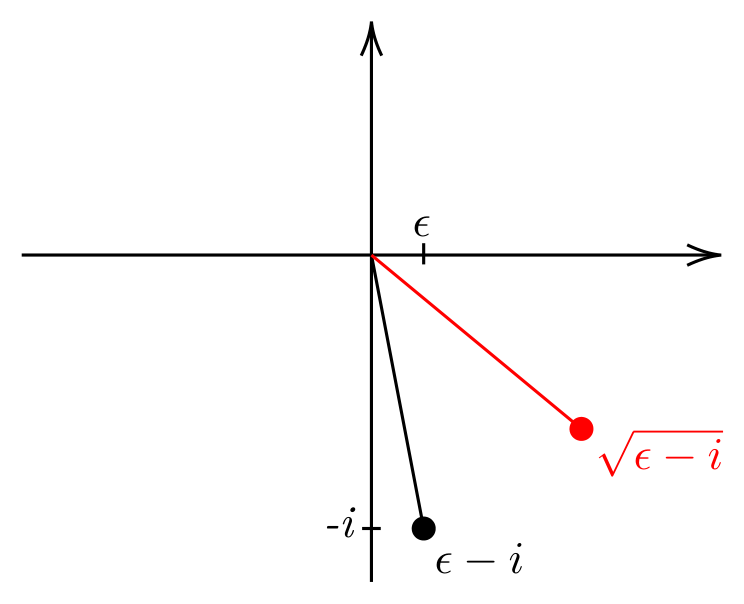
\includegraphics[width=0.72\textwidth]{figures/fig_p167_a.png}
\end{center}
% [图：原书 p.166，图内文字照原样保留]

由此得到
\[
\hat u=\lim_{\epsilon\to0^+}\hat u_\epsilon=\sqrt{2\pi}\,e^{\frac i4\pi}e^{-\frac i2\xi^2}.
\]
类似地，对 $v=e^{-\frac i2x^2}$，有
\[
\hat v=\lim_{\epsilon\to0^+}\frac{\sqrt{2\pi}}{\sqrt{\epsilon+i}}\,e^{-\frac{\xi^2}{2(\epsilon+i)}}
=\sqrt{2\pi}\,e^{-\frac i4\pi}e^{\frac i2\xi^2}.
\]
\begin{center}
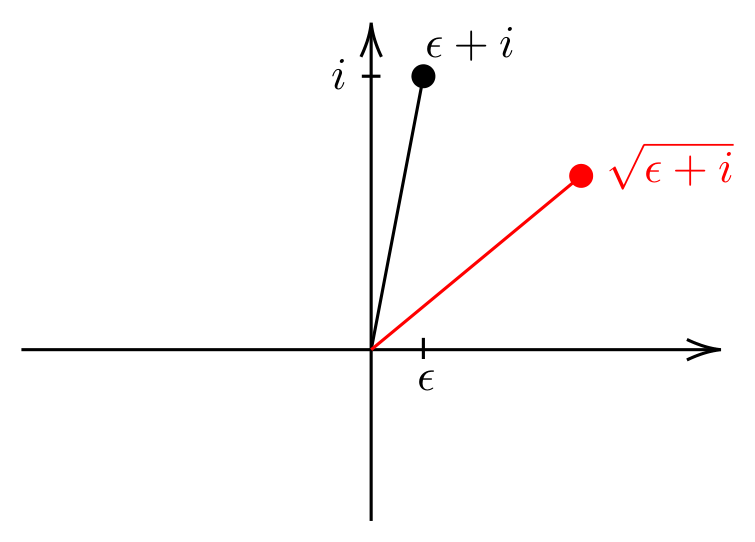
\includegraphics[width=0.62\textwidth]{figures/fig_p167_b.png}
\end{center}
% [图：原书 p.166，图内文字照原样保留]
\end{example}

对上例的计算稍作推广，便得到下述结果。细节留给读者。

\begin{proposition}{3.1.18}
设 $A$ 是实对称非奇异的 $n\times n$ 矩阵。则
\[
\mathcal{F}\left(e^{\frac i2A(x)}\right)
=\frac{(2\pi)^{n/2}}{\sqrt{|\det A|}}\,e^{\frac{i\pi}{4}\sgn(A)}e^{-\frac i2A^{-1}(\xi)},
\qquad\text{其中}\quad A(x)=\sum_{i,j=1}^n A_{ij}x^ix^j.
\]
这里 $\sgn(A)=\#\{\text{正本征值}\}-\#\{\text{负本征值}\}$ 是 $A$ 的\emph{符号差}（signature）。
\end{proposition}

% [原文 p.167]

\subsection{半经典傅里叶变换}

现在我们引入参数 $\hbar>0$。

\begin{definition}{3.1.19}
\emph{半经典傅里叶变换}（semi-classical Fourier transform）定义为
\[
\mathcal{F}_\hbar(\varphi)(\xi)=\int_{\R^n}e^{-\frac i\hbar\langle x,\xi\rangle}\varphi(x)\,dx,
\qquad\forall\,\varphi\in S(\R^n).
\]
\end{definition}

变换 $\mathcal{F}_\hbar$ 可以看作 $\mathcal{F}$ 的一个重标度版本，并像前面一样延拓到 $S'(\R^n)$。

\begin{theorem}{3.1.20}
半经典傅里叶变换给出同构
\[
\mathcal{F}_\hbar:S(\R^n)\longrightarrow S(\R^n),
\]
并且满足以下性质：

① \emph{傅里叶反演公式}
\[
\mathcal{F}_\hbar^{-1}(\psi)(x)=\frac{1}{(2\pi\hbar)^n}\int_{\R^n}e^{\frac i\hbar\langle x,\xi\rangle}\psi(\xi)\,d\xi.
\]

②
\[
\mathcal{F}_\hbar\bigl((D_{x}^\hbar)^\alpha\varphi\bigr)=\xi^\alpha\mathcal{F}_\hbar(\varphi),\qquad
\mathcal{F}_\hbar\bigl((-x)^\alpha\varphi\bigr)=(D_{\xi}^\hbar)^\alpha\mathcal{F}_\hbar(\varphi).
\]
这里
\[
D_{x^k}^\hbar:=\frac{\hbar}{i}\frac{\partial}{\partial x^k},
\qquad\text{以及}\qquad
(D_{x}^\hbar)^\alpha:=(D_{x^1}^\hbar)^{\alpha_1}\cdots(D_{x^n}^\hbar)^{\alpha_n}.
\]

③ \emph{等距性}
\[
\|\varphi\|_{L^2}=\frac{1}{(2\pi\hbar)^{n/2}}\|\mathcal{F}_\hbar(\varphi)\|_{L^2}.
\]
\end{theorem}

\begin{proposition}{3.1.21}（卷积）
有如下乘积公式：
\[
\mathcal{F}_\hbar(\varphi*\phi)=\mathcal{F}_\hbar(\varphi)\mathcal{F}_\hbar(\phi).
\]
这里
\[
\varphi*\phi(x)=\int_{\R^n}\varphi(x-y)\phi(y)\,dy
\]
是\emph{卷积}（convolution）。
\end{proposition}

\begin{proof}
\begin{align*}
(\mathcal{F}_\hbar(\varphi)\mathcal{F}_\hbar(\phi))(\xi)
&=\int_{\R^n}e^{-\frac i\hbar\langle x,\xi\rangle}\varphi(x)\,dx
\int_{\R^n}e^{-\frac i\hbar\langle y,\xi\rangle}\,dy\\
&=\int_{\R^n}\int_{\R^n}e^{-\frac i\hbar\langle x+y,\xi\rangle}\varphi(x)\phi(y)\,dxdy\\
&=\int_{\R^n}\int_{\R^n}e^{-\frac i\hbar\langle z,\xi\rangle}\varphi(x)\phi(z-x)\,dxdz\\
&=\mathcal{F}_\hbar(\varphi*\phi)(\xi).
\end{align*}
\tutornote{原文此行第一式的第二个积分漏写了被积函数 $\phi(y)$，下一行已补正，不影响结论。}
\end{proof}

% [原文 p.168]

\begin{proposition}{3.1.22}
设 $A$ 是实对称非奇异的 $n\times n$ 矩阵。则
\[
\mathcal{F}_{\hbar}\left(e^{\frac{i}{2\hbar}A(x)}\right)
=\frac{(2\pi\hbar)^{n/2}}{\sqrt{|\det A|}}\,e^{\frac{i\pi}{4}\sgn(A)}e^{-\frac{i\hbar}{2}A^{-1}(\xi)},
\qquad\text{其中}\quad A(x)=\sum_{i,j=1}^n A_{ij}x^ix^j.
\]
这里 $\sgn(A)=\#\{\text{正本征值}\}-\#\{\text{负本征值}\}$ 是 $A$ 的符号差。
\end{proposition}

\begin{proof}
由命题 3.1.18 作重标度 $x\to\frac{x}{\sqrt{\hbar}}$、$\xi\to\frac{\xi}{\sqrt{\hbar}}$ 即得。
\end{proof}

\takeaway{本节定义施瓦茨函数与缓增分布，建立傅里叶变换的反演、求导、周期性与共轭性质，证明普朗歇尔定理与卷积定理，并给出半经典标度下傅里叶变换的基本估计，为后面的量子化作准备。}

\section{施瓦茨象征的量子化}

遵循狄拉克的量子化原理，我们要找一个量子化过程
\[
Q:\mathrm{Obs}^{cl}\longrightarrow\mathrm{Obs}^{q},\qquad f\longmapsto\wh f,
\]
它把经典可观测对象 $f$（相空间上的函数）映为线性算子。

\subsection{量子化方案}

\paragraph{科恩–尼伦伯格量子化}
考虑标准相空间 $\R^{2n}$。

\begin{definition}{3.2.1}
给定 $a(x,\xi)\in S(\R^{2n})$，定义\emph{标准量子化}（standard quantization，或称\emph{科恩–尼伦伯格量子化}，Kohn–Nirenberg quantization）为作用在 $\varphi\in S(\R^n)$ 上的算子 $a^{KN}$：
\[
(a^{KN}\varphi)(x)
=\frac{1}{(2\pi\hbar)^n}\int_{\R^n}\int_{\R^n}e^{\frac i\hbar\langle x-y,\xi\rangle}a(x,\xi)\varphi(y)\,dyd\xi.
\]
\end{definition}

这是伪微分算子，我们常把它写成 $a^{KN}(x,D_{x}^\hbar)\varphi$。它也可以通过傅里叶变换解释为
\[
(a^{KN}\varphi)(x)=\mathcal{F}_\hbar^{-1}\bigl(a(x,\cdot)\mathcal{F}_\hbar(\varphi)\bigr).
\]
我们把它写成
\[
(a^{KN}\varphi)(x)=\int_{\R^n}K_a(x,y)\varphi(y)\,dy,
\]
其中
\[
K_a(x,y)=\frac{1}{(2\pi\hbar)^n}\int_{\R^n}e^{\frac i\hbar\langle x-y,\xi\rangle}a(x,\xi)\,d\xi
\]
是 $a^{KN}$ 的\emph{施瓦茨核}（Schwartz kernel）。这一表达式是一个部分傅里叶变换，它表明
\[
a^{KN}:S'(\R^n)\to S(\R^n)\qquad\text{当}\quad a\in S(\R^{2n}).
\]
此外，若 $a$ 本身是缓增分布，则 $K_a(x,y)$ 作为缓增分布也有意义。这时，核 $K_a$ 定义了映射
\[
K_a:S(\R^n)\longrightarrow S'(\R^n)\qquad\text{当}\quad a\in S'(\R^{2n}).
\]

% [原文 p.169]

\begin{proposition}{3.2.2}
给定缓增分布 $a(x,\xi)\in S'(\R^{2n})$，标准量子化定义了算子
\[
a^{KN}:S(\R^n)\longrightarrow S'(\R^n),
\]
其定义为
\[
(a^{KN}\varphi)(\psi)=\int_{\R^n}\int_{\R^n}\psi(x)K_a(x,y)\varphi(y)\,dydx.
\]
\end{proposition}

我们将直接沿用同一个公式
\[
(a^{KN}\varphi)(x)
=\frac{1}{(2\pi\hbar)^n}\int_{\R^n}\int_{\R^n}e^{\frac i\hbar\langle x-y,\xi\rangle}a(x,\xi)\varphi(y)\,dyd\xi
\]
来处理 $a\in S'(\R^{2n})$ 与 $\varphi\in S(\R^n)$。

\begin{example}{3.2.3}
设 $f(x)$ 是 $x$ 的函数。由显式公式可得
\[
(fa)^{KN}=f\cdot a^{KN}.
\]
这里 $f\cdot$ 表示乘以 $f(x)$ 的算子。与我们将要讨论的其他量子化相比，这是标准量子化特有的性质。特别地，若 $a(x,\xi)=a(x)$ 不依赖 $\xi$，则
\[
a^{KN}(x)\varphi=a(x)\varphi(x).
\]
\end{example}

\begin{example}{3.2.4}
考虑 $a=e^{\frac i\hbar\langle\lambda,\xi\rangle}$，其中 $\lambda\in\R^n$。可以把它看作缓增分布。则
\begin{align*}
(a^{KN}\varphi)(x)
&=\frac{1}{(2\pi\hbar)^n}\int_{\R^n}\int_{\R^n}e^{\frac i\hbar\langle x-y,\xi\rangle}e^{\frac i\hbar\langle\lambda,\xi\rangle}\varphi(y)\,dyd\xi\\
&=\int_{\R^n}\delta(x-y+\lambda)\varphi(y)\,dy\\
&=\varphi(x+\lambda).
\end{align*}
我们可以形式地把它写成
\[
\left(e^{\frac i\hbar\langle\lambda,\xi\rangle}\right)^{KN}
=e^{\frac i\hbar\langle\lambda,D_{x}^\hbar\rangle}
=e^{\langle\lambda,\frac{\partial}{\partial x}\rangle},
\]
由此得到物理学中广泛使用的公式
\[
e^{\langle\lambda,\frac{\partial}{\partial x}\rangle}\varphi(x)=\varphi(x+\lambda).
\]
对 $\lambda$ 求导，便得到
\[
(\xi^\alpha)^{KN}=(D_{x}^\hbar)^\alpha.
\]
这里 $D^\hbar_{x^k}:=\frac{\hbar}{i}\frac{\partial}{\partial x^k}$，$(D^\hbar_{x})^\alpha:=(D^\hbar_{x^1})^{\alpha_1}\cdots(D^\hbar_{x^n})^{\alpha_n}$，而 $\alpha=(\alpha_1,\cdots,\alpha_n)$ 是多重指标。公式 $(\xi^\alpha)^{KN}=(D_{x}^\hbar)^\alpha$ 也可以直接由傅里叶变换得到。
\end{example}

综合上面两个例子，我们得到下述结果。

\begin{proposition}{3.2.5}
设 $a(x,\xi)=\sum_{|\alpha|\le N}a_\alpha(x)\xi^\alpha$ 关于 $\xi$ 是多项式，则它的标准量子化为
\[
a^{KN}(x,D_{x}^\hbar)=\sum_{|\alpha|\le N}a_\alpha(x)(D_{x}^\hbar)^\alpha.
\]
\end{proposition}

% [原文 p.170]

这个命题说明：标准量子化把所有 $\xi$ 都放到右边，并把它们变成导数。这也称为\emph{正规排序}（normal ordering）。

\begin{proposition}{3.2.6}
设 $a(x,\xi)=e^{\frac i\hbar\langle x,\mu\rangle+\frac i\hbar\langle\lambda,\xi\rangle}$，$\mu,\lambda\in\R^n$。则
\[
(a^{KN}\varphi)(x)=e^{\frac i\hbar\langle x,\mu\rangle}\varphi(x+\lambda).
\]
\end{proposition}

换言之，我们有
\[
\left(e^{\frac i\hbar\langle x,\mu\rangle+\frac i\hbar\langle\lambda,\xi\rangle}\right)^{KN}
=e^{\frac i\hbar\langle x,\mu\rangle}e^{\frac i\hbar\langle\lambda,D_{x}^\hbar\rangle}
=e^{\frac i\hbar\langle x,\mu\rangle}e^{\langle\lambda,\frac{\partial}{\partial x}\rangle}.
\]

\paragraph{外尔量子化}
显然，量子化可以有不同的「排序」方案。保持酉性的对称方案称为\emph{外尔排序}（Weyl ordering）。

\begin{definition}{3.2.7}
给定 $a(x,\xi)\in S(\R^{2n})$，定义它的\emph{外尔量子化}（Weyl quantization）为作用在 $\varphi(x)\in S(\R^n)$ 上的算子 $a^W$：
\[
(a^W\varphi)(x)
=\frac{1}{(2\pi\hbar)^n}\int_{\R^n}\int_{\R^n}e^{\frac i\hbar\langle x-y,\xi\rangle}a\left(\frac{x+y}{2},\xi\right)\varphi(y)\,dyd\xi.
\]
\end{definition}

这是伪微分算子，我们常把它写成 $a^W(x,D_{x}^\hbar)\varphi$。相应的施瓦茨核是
\[
K_a^W(x,y)=\frac{1}{(2\pi\hbar)^n}\int_{\R^n}e^{\frac i\hbar\langle x-y,\xi\rangle}a\left(\frac{x+y}{2},\xi\right)d\xi.
\]
与前文一样，外尔量子化可延拓为
\[
a^W:S'(\R^n)\longrightarrow S(\R^n)\qquad\text{对}\quad a\in S(\R^{2n}),
\]
以及
\[
a^W:S(\R^n)\longrightarrow S'(\R^n)\qquad\text{对}\quad a\in S'(\R^{2n}).
\]
下面解释外尔量子化与对称排序的关系。

\begin{proposition}{3.2.8}
设 $a(x,\xi)=e^{\frac i\hbar\langle x,\mu\rangle+\frac i\hbar\langle\lambda,\xi\rangle}$，其中 $\mu,\lambda\in\R^n$。则
\[
(a^W\varphi)(x)=e^{\frac i\hbar\langle x,\mu\rangle+\frac{i}{2\hbar}\langle\lambda,\mu\rangle}\varphi(x+\lambda).
\]
\end{proposition}

这一公式可以形式地写成
\[
\left(e^{\frac i\hbar\langle x,\mu\rangle+\frac i\hbar\langle\lambda,\xi\rangle}\right)^{W}
=e^{\frac i\hbar\langle\mu,x\rangle+\langle\lambda,\frac{\partial}{\partial x}\rangle}
=e^{\frac i\hbar\langle\mu,x\rangle+\frac i\hbar\langle\lambda,D_{x}^\hbar\rangle}.
\]

\begin{proof}
\begin{align*}
(a^W\varphi)(x)
&=\frac{1}{(2\pi\hbar)^n}\int_{\R^n}\int_{\R^n}e^{\frac i\hbar\langle x-y+\lambda,\xi\rangle+\frac i\hbar\left\langle\frac{x+y}{2},\mu\right\rangle}\varphi(y)\,dyd\xi\\
&=\int_{\R^n}\delta(x-y+\lambda)e^{\frac i\hbar\left\langle\frac{x+y}{2},\mu\right\rangle}\varphi(y)\,dy\\
&=e^{\frac i\hbar\langle x,\mu\rangle+\frac{i}{2\hbar}\langle\lambda,\mu\rangle}\varphi(x+\lambda).
\end{align*}

% [原文 p.171]

这一公式可写成
\[
a^W=e^{\frac i\hbar\langle\mu,x\rangle+\frac{i}{2\hbar}\langle\mu,\lambda\rangle}e^{\langle\lambda,\frac{\partial}{\partial x}\rangle}
=e^{\frac i\hbar\langle\mu,x\rangle+\langle\lambda,\frac{\partial}{\partial x}\rangle},
\]
其中最后一步用了\emph{贝克–坎贝尔–豪斯多夫}（Baker–Campbell–Hausdorff）公式。
\end{proof}

\begin{definition}{3.2.9}
给定算子 $L_1,\cdots,L_m$，定义
\[
\operatorname{Sym}(L_1\cdots L_m)=\frac{1}{m!}\sum_{\sigma\in S_m}L_{\sigma(1)}\cdots L_{\sigma(m)}
\]
为它们乘积的\emph{对称排序}（symmetric ordering）。
\end{definition}

\begin{proposition}{3.2.10}
设 $a(x,\xi)\in\C[x,\xi]$ 是多项式。则
\[
a^W=\operatorname{Sym}\bigl(a(\hat{x},D_{x}^\hbar)\bigr).
\]
这里 $\hat x^k$ 是乘以 $x^k$ 的算子，$D^\hbar_{x^k}:=\frac{\hbar}{i}\frac{\partial}{\partial x^k}$。
\end{proposition}

\begin{proof}
由命题 3.2.8 对 $\mu,\lambda$ 作泰勒展开即得。形式地，
\[
\left(e^{\frac i\hbar\langle x,\mu\rangle+\frac i\hbar\langle\lambda,\xi\rangle}\right)^{W}
=e^{\frac i\hbar\langle\mu,x\rangle+\frac i\hbar\langle\lambda,D_{x}^\hbar\rangle}.
\]
于是泰勒展开给出对称排序。这一形式论证可以在傅里叶变换的演算中严格化。细节留给读者。
\end{proof}

\begin{example}{3.2.11}
考虑 $(x,\xi)\in\R^2$。
\begin{center}
\begin{tabular}{lll}
\toprule
相位函数 & 标准量子化 & 外尔量子化\\
\midrule
$x\xi$ & $xD^\hbar_x$ & $\frac12\left(xD^\hbar_x+D^\hbar_xx\right)$\\
$x^2\xi$ & $x^2D^\hbar_x$ & $\frac13\left(x^2D^\hbar_x+xD^\hbar_xx+D^\hbar_xx^2\right)=x^2D^\hbar_x+\frac{\hbar}{i}xD^\hbar_x$\\
\bottomrule
\end{tabular}
\end{center}
\end{example}

我们引入如下记号（见命题 3.2.8）：
\[
T_\hbar(\mu,\lambda)=\left(e^{\frac i\hbar\langle x,\mu\rangle+\frac i\hbar\langle\lambda,\xi\rangle}\right)^{W}:\quad
\varphi(x)\mapsto e^{\frac i\hbar\langle x,\mu\rangle+\frac{i}{2\hbar}\langle\lambda,\mu\rangle}\varphi(x+\lambda).
\]
这一显式公式表明 $T_\hbar(\mu,\lambda)$ 是酉算子。

给定 $a(x,\xi)\in S(\R^{2n})$，我们可以用傅里叶变换把它分解为
\[
a(x,\xi)=\frac{1}{(2\pi\hbar)^{2n}}\int_{\R^{2n}}\hat a(\mu,\lambda)e^{\frac i\hbar\langle x,\mu\rangle+\frac i\hbar\langle\lambda,\xi\rangle}\,d\mu\,d\lambda.
\]
由于 $T_\hbar(\mu,\lambda)$ 是酉算子且 $\hat a(\mu,\lambda)\in S(\R^{2n})$，积分
$\frac{1}{(2\pi\hbar)^{2n}}\int_{\R^{2n}}\hat a(\mu,\lambda)T_\hbar(\mu,\lambda)\,d\mu\,d\lambda$
收敛到一个线性算子，它恰好就是外尔量子化
\[
a^W=\frac{1}{(2\pi\hbar)^{2n}}\int_{\R^{2n}}\hat a(\mu,\lambda)T_\hbar(\mu,\lambda)\,d\mu\,d\lambda.
\]

% [原文 p.172]

\paragraph{一般量子化方案}
\begin{definition}{3.2.12}
一般地，对 $0\le t\le1$，定义量子化
\[
(\operatorname{Op}_t(a)\varphi)(x)
=\frac{1}{(2\pi\hbar)^n}\int_{\R^n}\int_{\R^n}e^{\frac i\hbar\langle x-y,\xi\rangle}a(tx+(1-t)y,\xi)\varphi(y)\,dyd\xi.
\]
\end{definition}

于是 $\operatorname{Op}_t(a)$ 给出算子
\[
\operatorname{Op}_t(a):S'(\R^n)\longrightarrow S(\R^n)\qquad\text{对}\quad a\in S(\R^{2n}),
\]
\[
\operatorname{Op}_t(a):S(\R^n)\longrightarrow S'(\R^n)\qquad\text{对}\quad a\in S'(\R^{2n}).
\]
形如 $\operatorname{Op}_t(a)$ 的算子称为\emph{半经典伪微分算子}（semiclassical pseudodifferential operator）。

\begin{itemize}[leftmargin=2.2em,itemsep=2pt]
\item $t=1$。$\operatorname{Op}_1(a)=a^{KN}$，即标准量子化。
\item $t=\frac12$。$\operatorname{Op}_{\frac12}(a)=a^W$，即外尔量子化。
\end{itemize}

对任意 $0\le t\le1$，有
\[
\begin{cases}
\operatorname{Op}_t(x^k)=\text{乘以 }x^k\text{ 的算子},\\[2pt]
\operatorname{Op}_t(\xi_j)=D^\hbar_{x^j}=\frac{\hbar}{i}\frac{\partial}{\partial x^j}.
\end{cases}
\]
特别地，\emph{正则对易关系}
\[
[\operatorname{Op}_t(x^k),\operatorname{Op}_t(\xi_j)]=i\hbar\delta^k_j
\]
总是成立。

\begin{example}{3.2.13}
考虑二次指数
\[
f(\xi)=e^{\frac{i}{2\hbar}A(\xi)}.
\]
这里 $A=(A_{ij})$ 是实对称非奇异的 $n\times n$ 矩阵，$A(\xi)=\sum_{i,j=1}^nA_{ij}\xi_i\xi_j$。由于 $f$ 不依赖 $x$，对一切 $0\le t\le1$ 都有 $\operatorname{Op}_t(f)=f^{KN}$。由命题 3.1.22，
\[
\mathcal{F}_\hbar^{-1}\bigl(e^{\frac{i}{2\hbar}A(\xi)}\bigr)
=\frac{e^{\frac{i\pi}{4}\sgn A}}{(2\pi\hbar)^{n/2}\sqrt{|\det A|}}\,e^{-\frac{i}{2\hbar}A^{-1}(x)}.
\]
因此
\begin{align*}
(f^{KN}\varphi)(x)
&=\frac{1}{(2\pi\hbar)^n}\int_{\R^n}\int_{\R^n}e^{\frac i\hbar\langle x-y,\xi\rangle}e^{\frac{i}{2\hbar}A(\xi)}\varphi(y)\,d\xi\,dy\\
&=\int_{\R^n}\mathcal{F}_\hbar^{-1}(f)(x-y)\varphi(y)\,dy\\
&=\frac{e^{\frac{i\pi}{4}\sgn A}}{(2\pi\hbar)^{n/2}\sqrt{|\det A|}}\int_{\R^n}e^{-\frac{i}{2\hbar}A^{-1}(y)}\varphi(x+y)\,dy.
\end{align*}
由于 $(\xi)^{KN}=D^\hbar_{x}=\hbar D_{x}$，我们形式地把这个公式写成
\[
e^{\frac{i\hbar}{2}A(D_{x})}\varphi(x)
=\frac{e^{\frac{i\pi}{4}\sgn A}}{(2\pi\hbar)^{n/2}\sqrt{|\det A|}}\int_{\R^n}e^{-\frac{i}{2\hbar}A^{-1}(y)}\varphi(x+y)\,dy.
\]
\end{example}

% [原文 p.173]

\subsection{$L^2$ 上的算子}

现在我们把具有施瓦茨象征的伪微分算子延拓为 $L^2(\R^n)$ 上的算子。

\begin{lemma}{3.2.14}（舒尔检验）
设 $A$ 是线性算子
\[
Au(x)=\int_{\R^n}K(x,y)u(y)\,dy,
\]
其施瓦茨核为 $K(x,y)$。假设
\[
C_1=\sup_{x}\int_{\R^n}|K(x,y)|\,dy<\infty,\qquad
C_2=\sup_{y}\int_{\R^n}|K(x,y)|\,dx<\infty.
\]
则对任意 $p\in[1,\infty]$ 与 $u\in L^p(\R^n)$，
\[
\|Au\|_{L^p}\le C_1^{1-\frac1p}C_2^{\frac1p}\|u\|_{L^p}.
\]
\end{lemma}

\begin{proof}
$p=\infty$ 的情形显然。设 $p\in[1,\infty)$。令 $\frac1p+\frac1q=1$。由 Hölder 不等式，
\begin{align*}
\int_{\R^n}|K(x,y)u(y)|\,dy
&=\int_{\R^n}|K(x,y)|^{\frac1q}\left|K(x,y)^{\frac1p}u(y)\right|\,dy\\
&\le\left(\int_{\R^n}|K(x,y)|\,dy\right)^{\frac1q}
\left(\int_{\R^n}|K(x,y)u^p(y)|\,dy\right)^{\frac1p}\\
&\le C_1^{\frac1q}\left(\int_{\R^n}|K(x,y)u^p(y)|\,dy\right)^{\frac1p}.
\end{align*}
于是
\begin{align*}
\|Au\|_{L^p}^p
&=\int_{\R^n}\left|\int_{\R^n}K(x,y)u(y)\,dy\right|^p dx\\
&\le C_1^{\frac pq}\int_{\R^n}\int_{\R^n}|K(x,y)u^p(y)|\,dydx\\
&\le C_1^{\frac pq}C_2\int_{\R^n}|u^p(y)|\,dy\\
&=C_1^{\frac pq}C_2\|u\|_{L^p}^p.
\end{align*}
\end{proof}

作为 $p=2$ 的特殊情形，我们有
\[
\|Au\|_{L^2}\le(C_1C_2)^{\frac12}\|u\|_{L^2}.
\]

\begin{theorem}{3.2.15}（有界性）
假设 $a\in S(\R^{2n})$。则 $a^W$ 定义了有界线性算子
\[
a^W:L^2(\R^n)\longrightarrow L^2(\R^n),
\]
并且
\[
\|a^W\|_{L^2\to L^2}\le C\sup_{x}\sup_{|\alpha|\le n+1}\int_{\R^n}|\partial_{\xi}^\alpha a(x,\xi)|\,d\xi,
\]
其中界关于 $\hbar$ 是一致的。
\end{theorem}

% [原文 p.174]

\begin{proof}
$a^W$ 的施瓦茨核是
\[
K_a^W(x,y)=\frac{1}{(2\pi\hbar)^n}\int_{\R^n}e^{\frac i\hbar\langle x-y,\xi\rangle}a\left(\frac{x+y}{2},\xi\right)d\xi.
\]
于是
\begin{align*}
\int_{\R^n}|K_a^W(x,y)|\,dy
&=\frac{1}{(2\pi\hbar)^n}\int_{\R^n}\left|\int_{\R^n}e^{-\frac i\hbar\langle y,\xi\rangle}a\left(x+\frac{y}{2},\xi\right)d\xi\right|dy\\
&=\frac{1}{(2\pi)^n}\int_{\R^n}\left|\int_{\R^n}e^{-i\langle y,\xi\rangle}a\left(x+\frac{\hbar y}{2},\xi\right)d\xi\right|dy\\
&=\frac{1}{(2\pi)^n}\int_{\R^n}\left|\int_{\R^n}\langle y\rangle^{n+1}e^{-i\langle y,\xi\rangle}a\left(x+\frac{\hbar y}{2},\xi\right)d\xi\right|\frac{dy}{\langle y\rangle^{n+1}}\\
&\le C\sup_{|\alpha|\le n+1}\sup_{x,y}\left|\int_{\R^n}y^\alpha e^{-i\langle y,\xi\rangle}a\left(x+\frac{\hbar y}{2},\xi\right)d\xi\right|\\
&\le C\sup_{x}\sup_{|\alpha|\le n+1}\left|\int_{\R^n}\partial^\alpha_{\xi}a(x,\xi)\,d\xi\right|.
\end{align*}
对 $\int_{\R^n}|K(x,y)|\,dx$ 有类似的估计。定理由舒尔检验得到。
\end{proof}

类似的论证表明，其他所有量子化都给出有界算子（关于 $\hbar$ 一致）：
\[
\operatorname{Op}_t(a):L^2(\R^n)\longrightarrow L^2(\R^n).
\]
下一个命题说明外尔量子化的一个优点。

\begin{proposition}{3.2.16}（伴随）
设 $\operatorname{Op}_t^*(a):L^2(\R^n)\to L^2(\R^n)$ 是 $\operatorname{Op}_t(a)$ 的伴随算子。则
\[
\operatorname{Op}_t^*(a)=\operatorname{Op}_{1-t}(\overline a).
\]
特别地，当 $a$ 为实值时 $a^W$ 自伴。
\end{proposition}

\begin{proof}
算子 $\operatorname{Op}_t(a)$ 的施瓦茨核是
\[
K_a^t(x,y)=\frac{1}{(2\pi\hbar)^n}\int_{\R^n}e^{\frac i\hbar\langle x-y,\xi\rangle}a(tx+(1-t)y,\xi)\,d\xi.
\]
对 $\varphi_1,\varphi_2\in L^2(\R^n)$，
\begin{align*}
\langle\varphi_1,\operatorname{Op}_t(a)\varphi_2\rangle_{L^2}
&=\int_{\R^n}\int_{\R^n}\overline{\varphi_1(x)}K_a^t(x,y)\varphi_2(y)\,dydx\\
&=\int_{\R^n}\int_{\R^n}\overline{K_a^{1-t}(y,x)}\varphi_1(x)\varphi_2(y)\,dydx\\
&=\langle\operatorname{Op}_{1-t}(\overline a)\varphi_1,\varphi_2\rangle_{L^2}.
\end{align*}
这表明 $\operatorname{Op}_t^*(a)=\operatorname{Op}_{1-t}(\overline a)$。特别地，对外尔量子化 $a^W=\operatorname{Op}_{\frac12}(a)$，
\[
(a^W)^*=(\overline a)^W.
\]
\end{proof}

% [原文 p.175]

\begin{theorem}{3.2.17}（紧性）
设 $a\in S(\R^{2n})$。则
\[
a^W:L^2(\R^n)\longrightarrow L^2(\R^n)
\]
是紧算子。
\end{theorem}

\begin{proof}
$a^W$ 的施瓦茨核
\[
K_a^W(x,y)=\frac{1}{(2\pi\hbar)^n}\int_{\R^n}e^{\frac i\hbar\langle x-y,\xi\rangle}a\left(\frac{x+y}{2},\xi\right)d\xi
\]
落在 $S(\R^{2n})$ 中，因为 $a\in S(\R^{2n})$，且 $K_a^W$ 本质上是 $a$ 的部分傅里叶变换。由速降性质，对任意多重指标 $\alpha,\beta$，
\begin{align*}
\sup_{x}\left|x^\alpha\partial^\beta_{x}(a^W\varphi)\right|
&\le\sup_{x,y}\left|x^\alpha\partial^\beta_{x}\langle y\rangle^N K_a^W(x,y)\right|\int_{\R^n}\langle y\rangle^{-N}|\varphi(y)|\,dy\\
&\le\sup_{x,y}\left|x^\alpha\partial^\beta_{x}\langle y\rangle^N K_a^W(x,y)\right|
\left(\int_{\R^n}\langle y\rangle^{-2N}\,dy\right)^{\frac12}\|\varphi\|_{L^2}\\
&\le C_{\alpha,\beta}\|\varphi\|_{L^2}\tag{$*$}
\end{align*}
其中 $N>\frac n2$。

现在设 $\{\varphi_k\}$ 是 $L^2(\R^n)$ 中任一有界序列。我们需要在 $L^2(\R^n)$ 中找到 $a^W(\varphi_k)$ 的收敛子列。固定 $N>\frac n2$，并定义
\[
\eta_k(x)=\langle x\rangle^N a^W(\varphi_k)(x).
\]
由于
\begin{align*}
\|a^W(\varphi_k)-a^W(\varphi_l)\|_{L^2}^2
&=\int_{\R^n}\langle x\rangle^{-2N}|\eta_k(x)-\eta_l(x)|^2dx\\
&\le\|\eta_k-\eta_l\|_{L^\infty}^2\int_{\R^n}\langle x\rangle^{-2N}dx\\
&=C\|\eta_k-\eta_l\|_{L^\infty}^2,
\end{align*}
只需证明 $\{\eta_k\}$ 的某个子列在 $L^\infty(\R^n)$ 中收敛。

设 $E\subset\R^n$ 是可数稠密子集。估计 $(*)$ 表明 $\{\eta_k\}$ 在 $L^\infty(\R^n)$ 中有界。因此，适当取子列后可设 $\{\eta_k(x)\}$ 对每个 $x\in E$ 收敛。下面证明 $\{\eta_k\}$ 是 $L^\infty$ 中的柯西列。这将推出 $\{\eta_k\}$ 的 $L^\infty$ 收敛性。

再次由估计 $(*)$，$\{|x|\eta_k\}$ 与 $\{\partial_{x}\eta_k\}$ 一致有界。对任意 $\varepsilon>0$，可以找到足够大的 $R>0$，使得
\[
|\eta_k(x)|\le\frac{\varepsilon}{2},\qquad\forall\,|x|>R,\ \forall k.
\]
因此在球外
\[
|\eta_k(x)-\eta_l(x)|\le\varepsilon,\qquad\forall\,|x|>R,\ \forall k.
\]
在球 $B_0(R)=\{x\in\R^n:|x|\le R\}$ 内（它是紧的），序列 $\{\eta_k\}$ 由估计 $(*)$ 一致有界且一致等度连续，而 $E$ 稠密。

% [原文 p.176]

可以找到有限个球 $\{B_{x_\alpha}(\delta)\}_{\alpha\in J}$，球心 $x_\alpha\in E$，半径 $\delta$ 足够小，使得
\[
B_0(R)\subset\bigcup_{\alpha\in J}B_{x_\alpha}(\delta),
\]
并且
\[
|\eta_k(x)-\eta_k(x_\alpha)|\le\frac{\varepsilon}{3},\qquad\text{对}\quad x\in B_{x_\alpha}(\delta).
\]
由于 $\{\eta_k(x_\alpha)\}_{k=1}^\infty$ 收敛，可以找到 $M>0$，使得
\[
|\eta_k(x_\alpha)-\eta_l(x_\alpha)|\le\frac{\varepsilon}{3},\qquad\forall\alpha\in J,\ \forall k,l\ge M.
\]
现在对任意 $|x|\le R$，取 $x_\alpha$ 使 $x\in B_{x_\alpha}(\delta)$，则对任意 $k,l\ge M$，
\[
|\eta_k(x)-\eta_l(x)|\le|\eta_k(x)-\eta_k(x_\alpha)|+|\eta_k(x_\alpha)-\eta_l(x_\alpha)|+|\eta_l(x_\alpha)-\eta_l(x)|\le\frac{\varepsilon}{3}+\frac{\varepsilon}{3}+\frac{\varepsilon}{3}=\varepsilon.
\]
综合球 $B_0(R)$ 内外的估计，可见 $\{\eta_k\}$ 是 $L^\infty(\R^n)$ 中的柯西列。
\end{proof}

\takeaway{本节引入量子化映射，给出科恩–尼伦伯格量子化与外尔量子化的核及基本性质，证明外尔量子化在 $L^2$ 上有界，并得到其伴随公式与紧性定理。}

\section{驻定相位与渐近展开}

我们常常需要理解带有快速振荡被积函数的积分，以及它们在半经典极限 $\hbar\to0$ 下的渐近行为。

\subsection{振荡积分}

\begin{definition}{3.3.1}
设 $f$ 是定义在 $(0,h_0]$（某 $h_0>0$）上的 $\hbar$ 的函数。若当 $\hbar\to0$ 时 $f$ 有\emph{渐近级数} $\sum_{k=0}^\infty a_k\hbar^k$，并记作
\[
f\sim\sum_{k=0}^\infty a_k\hbar^k,
\]
是指对每个 $N\in\Z_{\ge0}$，
\[
f-\sum_{k=0}^N a_k\hbar^k=O(\hbar^{N+1})\qquad\text{当}\quad\hbar\to0.
\]
若 $f\sim0$，即对一切 $N\in\Z_{\ge0}$ 都有 $f=O(\hbar^N)$，则称 $f=O(\hbar^\infty)$。
\end{definition}

\begin{definition}{3.3.2}
设 $a(x)\in C_c^\infty(\R^n)$，$\varphi(x)\in C^\infty(\R^n)$ 取实值。定义\emph{振荡积分}（oscillatory integral）
\[
I_\hbar=I_\hbar(a,\varphi)=\int_{\R^n}e^{\frac i\hbar\varphi(x)}a(x)\,dx,\qquad\hbar>0.
\]
\end{definition}

\begin{proposition}{3.3.3}
设 $K=\supp(a)$ 是紧集。假设 $d\varphi\ne0$ 于 $K$。则存在常数 $C$（只依赖于 $K$ 与 $\varphi$），使得对每个正整数 $N$，
\[
|I_\hbar|\le C\hbar^N\sum_{|\alpha|\le N}\sup_{\R^n}|\partial^\alpha a|
\]
成立。特别地，作为 $\hbar$ 的函数，有
\[
I_\hbar=O(\hbar^\infty)\qquad\text{当}\quad\hbar\to0.
\]
\end{proposition}

% [原文 p.177]

\begin{proof}
记 $|d\varphi|^2=\sum_{i=1}^n|\partial_i\varphi|^2$，由假设它在 $K$ 上处处不为零。考虑
\[
L=\frac{\hbar}{i}\frac{1}{|d\varphi|^2}\sum_{j=1}^n\partial_j\varphi\frac{\partial}{\partial x^j},\qquad x\in K,
\]
它满足
\[
L\left(e^{\frac i\hbar\varphi}\right)=e^{\frac i\hbar\varphi}.
\]
作分部积分可得
\[
I_\hbar=\int_{\R^n}L^N\left(e^{\frac i\hbar\varphi}\right)a\,dx=\int_{\R^n}e^{\frac i\hbar\varphi}(L^*)^N(a)\,dx,
\]
其中
\[
L^*(-)=-\frac{\hbar}{i}\sum_{j=1}^n\frac{\partial}{\partial x^j}\left(\frac{\partial_j\varphi}{|d\varphi|^2}\cdot(-)\right).
\]
命题由此直接得到。
\end{proof}

一般地，$d\varphi$ 可能在 $K$ 的某些点上为零，即
\[
\operatorname{Crit}(\varphi)\cap K\ne\varnothing.
\]
假设
\[
\operatorname{Crit}(\varphi)\cap K=\{p_1,p_2,\cdots,p_m\}
\]
是有限集。设 $U_i$ 是 $p_i$ 的小邻域，使得 $\{U_1,\cdots,U_m\}$ 互不相交。
\begin{center}
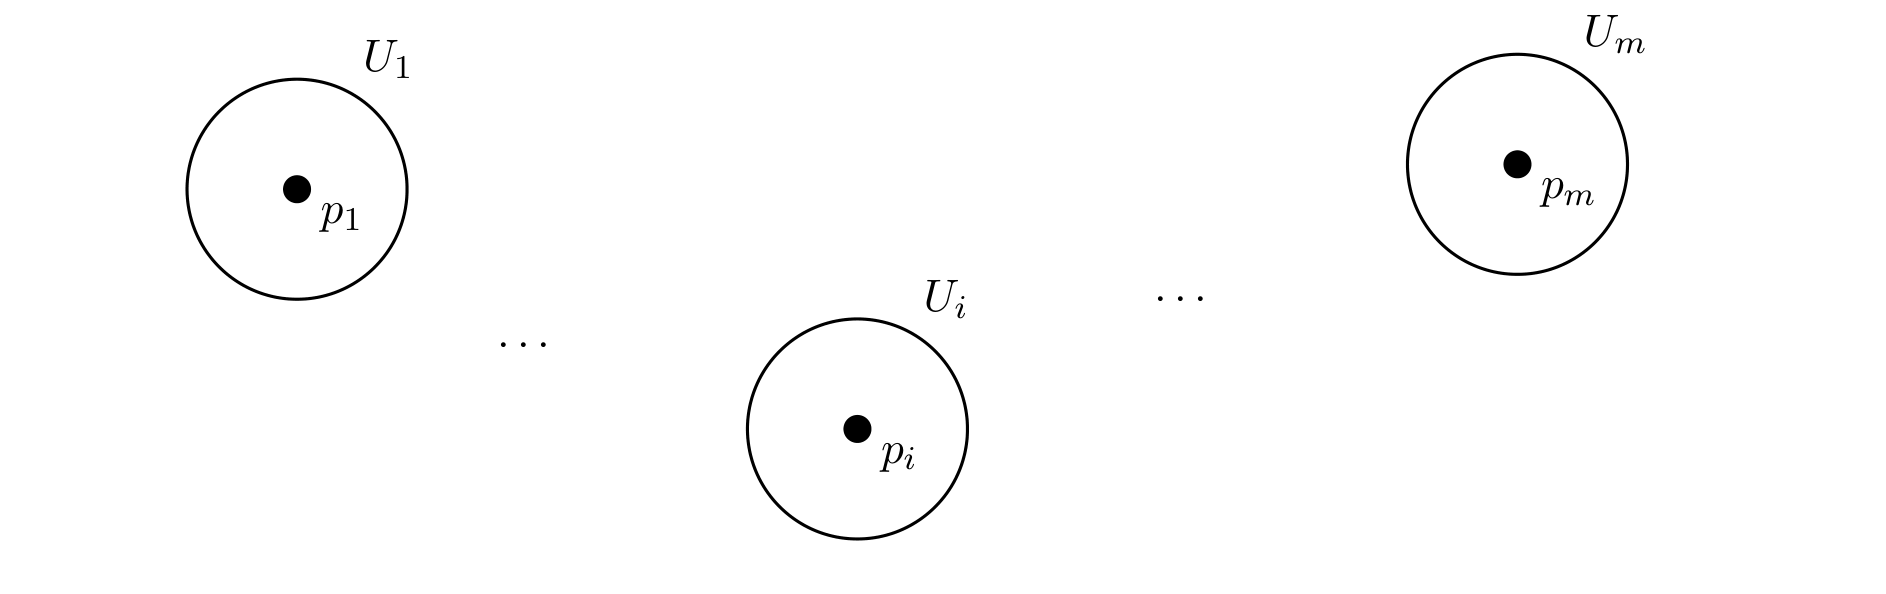
\includegraphics[width=0.72\textwidth]{figures/fig_p178_a.png}
\end{center}
% [图：原书 p.177，图内文字照原样保留]

选取截断函数 $0\le\chi_i\le1$，满足
\[
\begin{cases}
\chi_i=0 & \text{在 }U_i\text{ 外},\\
\chi_i=1 & \text{在 }p_i\text{ 的某个小邻域内}.
\end{cases}
\]
令 $\chi_0=1-(\chi_1+\cdots+\chi_m)$，它在每个 $p_i$ 附近为零。于是振荡积分可表示为
\[
I_\hbar=\int_{\R^n}e^{\frac i\hbar\varphi}\chi_0a\,dx+\sum_{j=1}^m\int_{\R^n}e^{\frac i\hbar\varphi}\chi_ja\,dx.
\]

% [原文 p.178]

由于 $d\varphi\ne0$ 于 $\supp(\chi_0a)$，由命题 3.3.3，
\[
\int_{\R^n}e^{\frac i\hbar\varphi}\chi_0a\,dx=O(\hbar^\infty)\qquad\text{当}\quad\hbar\to0.
\]
因此当 $\hbar\to0$ 时，$I_\hbar$ 的渐近行为完全由各个
\[
\int_{\R^n}e^{\frac i\hbar\varphi}\chi_ja\,dx
\]
决定，它们现在都局部化在临界点 $p_j$ 附近。

为理解局部贡献，下述莫尔斯引理起关键作用。

\begin{theorem}{3.3.4}
设 $\varphi:M\to\R$ 是光滑流形 $M$ 上的光滑函数，在 $p\in M$ 处有\emph{非退化临界点}（non-degenerate critical point）。则存在 $p$ 的某邻域内的局部坐标系 $\{x^1,\cdots,x^n\}$，使得
\[
\varphi(x)=\varphi(p)+\frac12\left((x^1)^2+\cdots+(x^r)^2-(x^{r+1})^2-\cdots-(x^n)^2\right).
\]
这里 $r=\#\{\operatorname{Hess}\varphi(p)\text{ 的正本征值}\}$。
\end{theorem}

莫尔斯引理说明：适当换坐标后，非退化临界点附近的相位函数可以化为二次表达式。

\begin{proposition}{3.3.5}
设 $a(x)\in C_c^\infty(\R^n)$，$\varphi(x)=\frac12A(x)=\frac12\sum_{i,j=1}^nA_{ij}x^ix^j$，其中 $(A_{ij})$ 是实对称非奇异矩阵。则有渐近展开
\[
\int_{\R^n}e^{\frac i{2\hbar}A(x)}a(x)dx\sim(2\pi\hbar)^{\frac n2}\frac{e^{\frac{i\pi}{4}\sgn A}}{\sqrt{|\det A|}}\left(\sum_{k=0}^\infty\frac{\hbar^k}{k!}\left(\frac{A^{-1}(D)}{2i}\right)^k a(0)\right).
\]
这里 $A^{-1}(D)=\sum_{i,j=1}^n(A^{-1})^{ij}D_iD_j$，而 $A^{-1}$ 是 $A$ 的逆矩阵。
\end{proposition}

\begin{proof}
由傅里叶变换，
\[
\int_{\R^n}e^{\frac i\hbar\varphi(x)}a(x)dx=\frac{1}{(2\pi)^n}\int_{\R^n}\widehat{\left(e^{-\frac i\hbar\varphi}\right)}(\xi)\hat a(\xi)d\xi.
\]
这里 $\widehat{(-)}=\mathcal F(-)$ 是傅里叶变换。由命题 3.1.18，
\[
\mathcal F\left(e^{-\frac i{2\hbar}A(x)}\right)=\frac{(2\pi\hbar)^{n/2}}{\sqrt{|\det A|}}e^{-\frac{i\pi}{4}\sgn(A)}e^{\frac{i\hbar}{2}A^{-1}(\xi)}.
\]
于是
\[
\int_{\R^n}e^{\frac i{2\hbar}A(x)}a(x)dx=\left(\frac{\hbar}{2\pi}\right)^{\frac n2}\frac{e^{\frac{i\pi}{4}\sgn(A)}}{\sqrt{|\det A|}}\int_{\R^n}e^{-\frac{i\hbar}{2}A^{-1}(\xi)}\hat a(\xi)d\xi.
\]
记
\[
J(\hbar,a)=\int_{\R^n}e^{-\frac{i\hbar}{2}A^{-1}(\xi)}\hat a(\xi)d\xi.
\]

% [原文 p.179]

则
\begin{align*}
\partial_\hbar J&=\int_{\R^n}e^{-\frac{i\hbar}{2}A^{-1}(\xi)}\frac{A^{-1}(\xi)}{2i}\hat a(\xi)d\xi\\
&=\int_{\R^n}e^{-\frac{i\hbar}{2}A^{-1}(\xi)}\frac{1}{2i}\widehat{\left(A^{-1}(D)a\right)}(\xi)d\xi\\
&=J\left(\hbar,\frac{A^{-1}(D)}{2i}a\right).
\end{align*}
将它用于泰勒展开，得
\[
J(\hbar,a)=\sum_{k=0}^{N-1}\frac{\hbar^k}{k!}J\left(0,\left(\frac{A^{-1}(D)}{2i}\right)^ka\right)+\frac{\hbar^N}{N!}R_N(\hbar,a),
\]
其中余项为
\[
R_N(\hbar,a)=N\int_0^1(1-t)^{N-1}\partial_\hbar^NJ(t\hbar,a)=N\int_0^1(1-t)^{N-1}J\left(t\hbar,\left(\frac{A^{-1}(D)}{2i}\right)^Na\right).
\]
由傅里叶积分公式，
\[
J\left(0,\left(\frac{A^{-1}(D)}{2i}\right)^ka\right)=(2\pi)^n\left(\frac{A^{-1}(D)}{2i}\right)^ka(0).
\]
利用
\[
\|\hat\varphi\|_{L^1}=\int_{\R^n}\hat\varphi(\xi)\langle\xi\rangle^{n+1}\langle\xi\rangle^{-(n+1)}d\xi\le C\left\|\hat\varphi(\xi)\langle\xi\rangle^{n+1}\right\|_{L^\infty}\le C\sup_{|\alpha|\le n+1}\|\partial^\alpha\varphi\|_{L^1},
\]
余项被控制为
\[
|R_N|\le C'_N\left\|\widehat{\left(A^{-1}(D)\right)^Na}\right\|_{L^1}\le C_N\sup_{|\alpha|\le2N+n+1}\|\partial^\alpha a\|_{L^1}.
\]
命题证毕。
\end{proof}

\subsection{驻定相位法}

\begin{theorem}{3.3.6}
设 $a\in C_c^\infty(\R^n)$，$\varphi\in C^\infty(\R^n)$，且
\[
\operatorname{Crit}(\varphi)\cap\supp(a)=\{x_0\},
\]
其中 $x_0$ 是 $\varphi$ 的非退化临界点。则存在阶数 $\le2k$ 的微分算子 $A_{2k}(x,D)$，使得有渐近展开
\[
\int_{\R^n}e^{\frac i\hbar\varphi}a\,dx\sim(2\pi\hbar)^{\frac n2}\left(\sum_{k=0}^\infty\hbar^kA_{2k}(x,D)a(x_0)\right)e^{\frac i\hbar\varphi(x_0)}.
\]
首项由下式给出：
\[
A_0=\frac{e^{\frac i4\pi\sgn\partial^2\varphi(x_0)}}{\sqrt{|\det\partial^2\varphi(x_0)|}},
\]
其中 $\partial^2\varphi(x_0)$ 表示矩阵 $(\partial_i\partial_j\varphi(x_0))$。
\end{theorem}

% [块界：本节（§3.3.2 驻定相位法）起于本页末；定理 3.3.6 的证明自 PDF p.181（原书 p.180）起，由 ch03b 接着译。本块止于定理 3.3.6 陈述，未写本节 \takeaway（§3.3 跨块，takeaway 归 ch03b）。原书 p.179 至此结束。]
